\chapter{The Syntactic Parsing Pipeline}
\label{ch:syntax}

\section{From Surface Form to Logical Form}

The Logical Random Field operates over propositions---but natural language arrives as strings. This chapter describes the pipeline from surface text to the key-value logical forms consumed by the LRF.

\section{A Key-Value Calculus}

Traditional first-order logic imposes arbitrary positional order on arguments:
\begin{equation}
\text{wrote}_{\text{arg0:PER}, \text{arg1:BOOK}}(c_{\text{Shakespeare}}, c_{\text{Macbeth}})
\end{equation}

We adopt a key-value formalism closer to dependency structure:
\begin{equation}
(\textsc{wrote}, \{\textsc{arg0}: c_{\text{Shakespeare}}, \textsc{arg1}: c_{\text{Macbeth}}\})
\end{equation}

This eliminates spurious ordering while preserving semantic content.

\section{Dependency Parsing}

Given a sentence like ``John sent a letter to Sally,'' dependency parsing yields:

\begin{center}
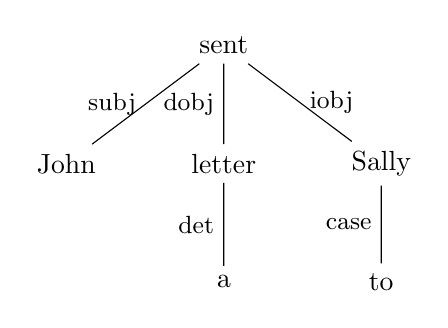
\begin{tikzpicture}[level distance=1.5cm, sibling distance=2cm]
\node {sent}
    child {node {John} edge from parent node[left] {\small subj}}
    child {node {letter} 
        child {node {a} edge from parent node[left] {\small det}}
        edge from parent node[left] {\small dobj}}
    child {node {Sally} 
        child {node {to} edge from parent node[left] {\small case}}
        edge from parent node[right] {\small iobj}};
\end{tikzpicture}
\end{center}

From this we extract:
\begin{equation}
(\textsc{send}, \{\textsc{subj}: \text{John}, \textsc{dobj}: \text{letter}, \textsc{iobj}: \text{Sally}\})
\end{equation}

\section{Entity Resolution}

Constants reference specific entities with types:
\begin{equation}
c_{\text{usa}} = \text{constant}(\text{USA}, \textsc{country})
\end{equation}

Entity resolution maps surface mentions to canonical constants in the knowledge base.

\section{Pipeline Architecture}

The full pipeline consists of:
\begin{enumerate}
    \item \textbf{Tokenization}: Segment text into tokens
    \item \textbf{Dependency Parsing}: Extract labeled dependency structure
    \item \textbf{Semantic Role Labeling}: Map dependencies to semantic roles
    \item \textbf{Entity Linking}: Resolve mentions to constants
    \item \textbf{Proposition Construction}: Build key-value logical forms
\end{enumerate}

Each stage admits both neural and symbolic implementations, with the LRF providing a consistent target representation.